%情報処理学会全国大会原稿テンプレート ver. 1.2

\documentclass[uplatex,twocolumn]{jsarticle}
\usepackage[top=30mm,bottom=25mm,left=20mm,right=20mm]{geometry}
\usepackage[T1]{fontenc}
\usepackage{txfonts}
\usepackage[expert,deluxe]{otf}
\usepackage[dvipdfmx,hiresbb]{graphicx}
\usepackage[dvipdfm]{hyperref}
\usepackage{pxjahyper}
\usepackage{multicol}
\setlength{\columnsep}{7mm}

\title{\vspace{-10mm}\Large{SNSにおいてフェイクニュースを拡散するユーザの特徴抽出}\footnotemark[0]}%要修正
\author{\large{岩橋 瑠伊\footnotemark[2]\qquad 矢吹 太朗}\\千葉工業大学 社会システム科学部 プロジェクトマネジメント学科\footnotemark[3]}%要修正
\date{}
\pagestyle{empty}
\begin{document}
\twocolumn[\maketitle]

\begingroup
\def\thefootnote{\fnsymbol{footnote}}
\footnotetext[0]{Feature extraction of users spreading fake news in SNS.}%要修正(最後はピリオド)
\footnotetext[2]{Rui Iwahashi (\verb|MAIL|)}%要修正
\footnotetext[3]{Department of Project Management, Faculty of Social Systems Science, Chiba Institute of Technology.}
\endgroup

\section{序論}
近年FacebookやTwitterを始めとしたマイクロブログがスマートフォンなどの普及と共に急激に普及している.Twitterは140字以内で記事(Tweet)を投稿するシンプルな構造であり,リアルタイム性と情報の強い伝播力をもつ.中でも,リツイート は他のユーザのTweetを引用し,情報を伝播させるものであり,Twitter特有の重要な機能である\cite{dema1}.

Twitterは2011年3月11日に発生した東日本大震災時に,携帯電話がつながらない状況下での有用な連絡手段として活躍した.しかし,その有用性はデマや誤情報も大量に拡散させる手助けとなりえる.実際に東日本大震災時に,数十種類のデマや誤情報が情報として拡散されてしまい,日本中を混乱させた.震災時のように連絡手段が限られた状況はこれからも発生する可能性は十分にあり,対策が必要である\cite{dema2}.

本研究では,デマが拡散されることを防ぐためにデマツイートをリツイートしているユーザーの特徴抽出を行う.デマツイートがリツイートされる原因として,デマをデマと見抜けないユーザー,面白半分でリツイートしているユーザーの2種類がいると考えた.この2種類のユーザーと,それ以外のユーザーにはTwitterの使い方に違いがあるのではないかと考えた.

\section{目的}
デマが拡散されることを防ぐために,デマツイートをリツイートしているユーザーの特徴抽出を行う.そのために,現時点でデマだとわかっているツイートを過去に拡散したユーザの活動履歴を収集・分析する.分析結果をランダムサンプリングしたデータと比較することで,デマを拡散するようなユーザに共通する特徴を抽出し,その結果を報告する.

\section{手法}
デマツイートをリツイートするユーザーとそれ以外のユーザーの違いを見つけ,その違いが偶然生じたものではないことを示すために以下の手法で研究する.
\begin{enumerate}
\item TwitterAPIを用いて日本人ユーザー50人をランダムサンプリングする.
\item TwitterAPIを用いてデマツイートをリツイートしたユーザー50人を取得する.
\item TwitterAPIを用いて集めた各ユーザーの最新100ツイートに含まれるリツイートの数を調べて,平均を計算する.
\item 日本人ユーザー50人とデマツイートをリツイートしたユーザー50人の最新100ツイートに含まれるリツイートの数の平均の差が,偶然的な誤差の範囲にあるものかどうかを判断する為に2標本T検定\cite{T}を行う.
\end{enumerate}

\section{結果}
TwitterAPIを用いて日本人ユーザー50人をランダムサンプリングした.4つのデマツイートからそれぞれ50人のリツイートユーザーを取得した.ランダムサンプリングした日本人ユーザー50人の平均リツイート数は20.04人,デマツイート1の平均リツイート数は56.68人,デマツイート2の平均リツイート数は62.64人,デマツイート3の平均リツイート数は58.46人となった,デマツイート4のの平均リツイート数は57.92人となった.デマツイート1と日本人ユーザー,デマツイート2と日本人ユーザー,デマツイート3と日本人ユーザー,デマツイート4と日本人ユーザーのそれぞれ3組には対応がないデータなので,F検定を行い分散が等しいか等しくないかを確かめる.等分散の場合の2標本T検定と不等分散の場合のT検定をF検定の結果に沿って行った結果,全ての組み合わせで有意差が確認できた.以下にデマツイート1から4のヒストグラムを示す.

\begin{figure}[htbp]
\centering
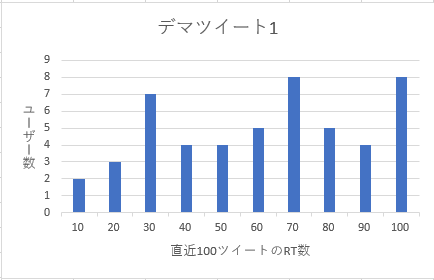
\includegraphics[clip,width=8.0cm]{d1.png}
\caption{デマツイート1のヒストグラム}
\label{ヒストグラム1}
\end{figure}

\begin{figure}[htbp]
\centering
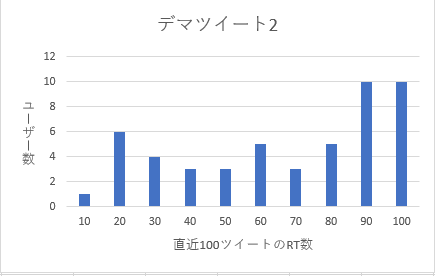
\includegraphics[clip,width=8.0cm]{d2.png}
\caption{デマツイート2のヒストグラム}
\label{ヒストグラム2}
\end{figure}

\begin{figure}[htbp]
\centering
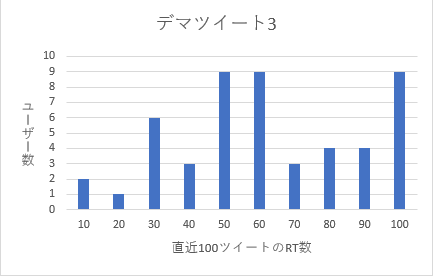
\includegraphics[clip,width=8.0cm]{d3.png}
\caption{デマツイート3のヒストグラム}
\label{ヒストグラム3}
\end{figure}

\begin{figure}[h]
\centering
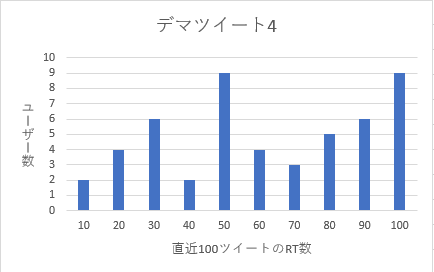
\includegraphics[clip,width=8.0cm]{d4.png}
\caption{デマツイート4のヒストグラム}
\label{ヒストグラム4}
\end{figure}

\section{考察}
デマを拡散するようなユーザに共通する特徴として,リツイート数に着目しランダムサンプリングしたユーザーとデマツイートをリツイートしたユーザーで直近100リツイート内のリツイート数を調査した結果,大きく数値が異なった.この結果からデマを拡散するようなユーザーはリツイート機能を多用する傾向にあり,ツイート内容の真偽を確かめる前にリツイートをし,デマ拡散者の一員となっていると考えられる.

自分がデマ拡散者にならない為の手段として,デマ拡散ユーザーリストにあるユーザーと,リツイートの多いユーザーを排除することが有効だと考えられる.

\section{結論}
本研究では,デマが拡散されることを防ぐために,デマツイートをリツイートしているユーザーの特徴抽出としてリツイート数の調査を行った.その結果,デマツイートを拡散するユーザーの特徴としてリツイート数が多いことを証明することができた.データ数が少ないことは否めないが,T検定の結果からデータの整合性は高いものと判断できる.本研究のデータを利用し,リツイート数以外のデータ(ツイート数,フォロー数,フォロワー数)などからもデマ拡散者の特徴を抽出し,更なる精度の向上とデータ数の増加に期待される.

\bibliographystyle{junsrt}
\bibliography{biblio}%「biblio.bib」というファイルが必要.

\end{document}